\section{Overview}

My expertise encompasses applied and computational mathematics, scientific computing, and computational physics. 
I am particularly focused on developing efficient numerical algorithms for modeling and simulating complex systems, with an emphasis on high-performance implementation. 
Specifically, I am working on \textbf{fast summation algorithms} designed for long-range interactions in doubly periodic systems, particularly in their application to molecular dynamics simulations. 
Additionally, I have a keen interest in \textbf{tensor network based algorithms} and their application in solving combinatorial optimization problems.
In these projects, I focused on designing new algorithms and their high-performance implementation across various platforms, including both CPU and GPU architectures, and accelerating them through modern parallel and distributed computing techniques.
% My current research focuses on 

In the following parts, I present an overview of my past and current work, emphasizing my research contributions and achievements, while also outlining my future research plans that aim to integrate applied mathematics with scientific exploration.

\section{Research Accomplishments}

\begin{figure}[h]
    \centering
    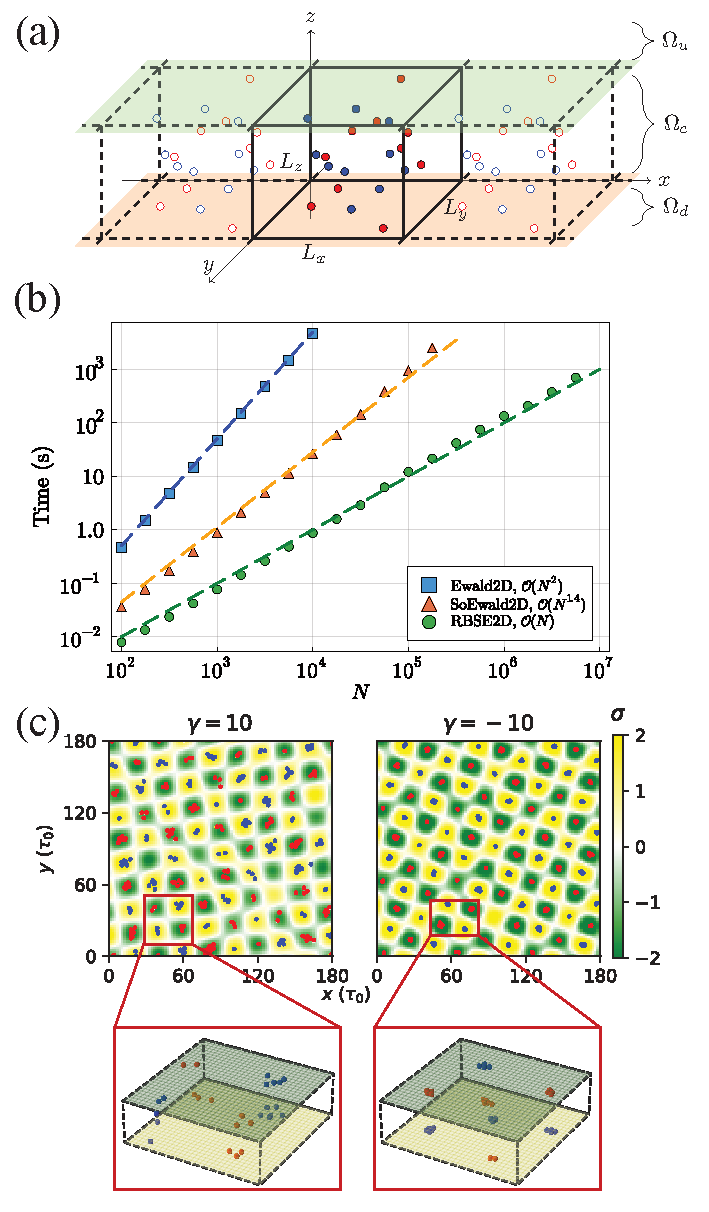
\includegraphics[width=0.45\textwidth]{figs/Q2D_onec.pdf}
    \caption{(a) Illustration of a doubly periodic charged system. (b) The scaling of the SOEwald2D method~\cite{gan2024fast}, which shows that with the random batch sampling technique, the method (RBSE2D) can achieve linear complexity. (c) The SSB phenomenon in the system with strong negative dielectric confinement~\cite{gao2024broken}, showing the checkerboard pattern formation of the surface charge density and the ion distribution.}
    \label{fig:Q2D}
\end{figure}

% In the subsequent sections, I will provide an brief overview of my additional work and contributions.

\subsection{Fast summation algorithms}

In my previous works, I focused on the fast summation algorithms for quasi-2D systems, which are three-dimensional systems exhibiting periodicity in only two dimensions as shown in \Cref{fig:Q2D} (a).
They are ubiquitous in nature, e.g. charged colloidal suspensions, liquid crystals, and biological systems.
However, simulating these systems is challenging due to the long range nature of the electrostatic interactions and the doubly-periodic boundary conditions, thus the fast summation algorithms for such systems are highly desirable.
Throughout my Ph.D. studies, I developed a range of innovative methods to address these systems, which will be detailed in the subsequent sections.

\textbf{The fast sum-of-Exponential Ewald2D method.}
Building on the success of the fast Gaussian transform via the sum-of-Exponential (SOE) approximation~\cite{Greengard2022ApproximatingTG}, I integrated the SOE approximation with the Ewald splitting technique to derive an accurate quasi-2D lattice summation formula with a complexity of~$O(N^{1.4})$ called the SOEwald2D method~\cite{gan2024fast}. 
This method is numerically stable and maintains its accuracy regardless of the system's thickness. 
Furthermore, the method is enhanced by employing a random batch sampling technique, which achieves linear complexity, as shown in \Cref{fig:Q2D} (b).
It has been demonstrated that a speedup of $2 \sim 3$ orders of magnitude comparing with Ewald2D method, enabling molecular dynamics (MD) simulations with up to $10^6$ particles on a single CPU core.
My contributions include the derivation of the quasi-2D lattice summation formula, the implementation of the method (see \href{https://github.com/HPMolSim/SoEwald2D.jl}{\texttt{SoEwald2D.jl}}), and the execution of related numerical tests.

\textbf{The fast sum-of-Gaussian method.}
To further enhance both the efficiency and accuracy of the fast summation methods for quasi-2D charged systems, my collaborators and I developed a spectral method that leverages the sum-of-Gaussian (SOG) expansion in conjunction with fast Fourier transforms.
The fast sum-of-Gaussian method~\cite{fssog} is a spectral method based on the sum-of-Gaussian (SOG) expansion and fast Fourier transform, where we integrate SOG expansion with a novel Fourier-Chebyshev solver to develop a fast summation method that achieves a complexity of $\mathcal{O}(N \log N)$ per time step.
Utilizing the SOG approach allows for a significant reduction in the required mesh resolution, down to approximately $60\%$ of that needed by the Ewald-based methods, without necessitating upsampling. 
This method is also highly effective for systems with large aspect ratios, accommodating ratios of up to $L_{x/y} / L_z = 10^{3.5}$ without incurring additional computational costs. 
My contributions primarily involved the implementation of this method, which includes a highly efficient particle-mesh solver \href{https://github.com/HPMolSim/ChebParticleMesh.jl}{\texttt{ChebParticleMesh.jl}} as a backend (similar to the \href{https://finufft.readthedocs.io/en/latest/}{\texttt{FINUFFT}} package), along with the Fourier-Chebyshev solver \href{https://github.com/HPMolSim/FastSpecSoG.jl}{\texttt{FastSpecSoG.jl}}. 
The resulting implementation is both efficient and scalable, capable of calculating long-range electrostatic interactions in quasi-2D systems with $10^6$ particles on a single CPU core in less than $10$ seconds.
Additionally, I conducted related numerical tests and collaborated on the algorithm design.

\textbf{The spontaneous symmetry breaking in doubly periodic charged systems.}
We developed stochastic methods to investigate doubly periodic charged systems with dielectric mismatches~\cite{quasiewald, gan2024random}. 
By employing appropriate singular subtraction techniques, this method can be effectively applied to systems exhibiting negative dielectric confinement. 
The findings indicate that SSB occurs in systems with strongly polarizable dielectric confinement~\cite{gao2024broken}, leading to the formation of checkerboard patterns as ions aggregate due to the strong polarization at the dielectric boundary as shown in \Cref{fig:Q2D} (c).
This work includes a prediction of the spontaneous symmetry breaking (SSB) phenomenon, detailing the conditions for lattice formation and the \textit{wavelength} of the checkerboard patterns, which have been validated through molecular dynamics simulations.
My contributions include the derivation and the implementation of the method (see \href{https://github.com/HPMolSim/QuasiEwald.jl}{\texttt{QuasiEwald.jl}}), and the study of the SSB phenomenon via MD simulations.

% Currently, I am working on further extending the spectral methods to systems with more complex boundary conditions, including the systems only periodic in one direction, and the systems with mixed boundary conditions.

\subsection{Tensor network based algorithms}

\begin{figure}[h]
    \centering
    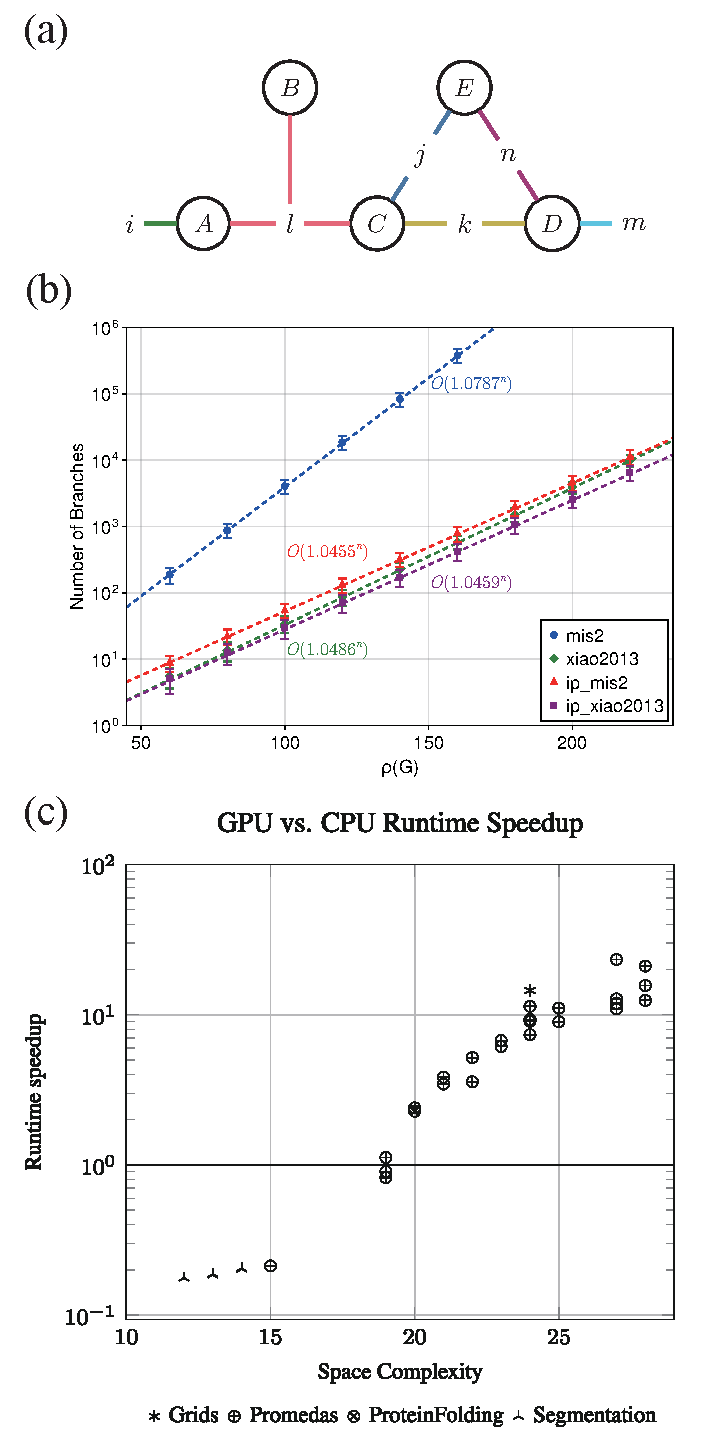
\includegraphics[width=0.45\textwidth]{figs/tn_onec.pdf}
    \caption{(a) Illustration of a simple tensor network, where the white circles represent the tensor nodes and the lines represent the indices. (b) Number of branches of the optimal branching algorithm (\texttt{ip\_mis2} and \texttt{ip\_xiao2013}) compared with the traditional branching algorithms (\texttt{mis2} and \texttt{xiao2013}), $\rho(G)$ represents the number of vertices here. (c) Speedup of the GPU accelerated inference algorithm compared to the CPU version.}
    \label{fig:tn}
\end{figure}

\begin{table*}[!htb]
    \centering
    \begin{tabular}{|l|l|}
        \hline
        \textbf{Project} & \textbf{Description} \\
        \hline
        \href{https://github.com/HPMolSim/ExTinyMD.jl}{\texttt{ExTinyMD.jl}} & A basic framework for simulating the particle systems. \\
        \hline
        \href{https://github.com/HPMolSim/EwaldSummations.jl}{\texttt{EwaldSummations.jl}} & Implementations of various Ewald summation based methods. \\
        \hline
        \href{https://github.com/HPMolSim/ChebParticleMesh.jl}{\texttt{ChebParticleMesh.jl}} & A particle-mesh solver for Poisson's equations for arbitrary dimensions and periodicity. \\
        \hline
        \href{https://github.com/TensorBFS/TropicalNumbers.jl}{\texttt{TropicalNumbers.jl}} & Implementation of the tropical semiring. \\
        \hline
        \href{https://github.com/TensorBFS/CuTropicalGEMM.jl}{\texttt{CuTropicalGEMM.jl}} & A GPU implementation of the general matrix multiplication of tropical semiring. \\
        \hline
        \href{https://github.com/ArrogantGao/TreeWidthSolver.jl}{\texttt{TreeWidthSolver.jl}} & A solver for the exact tree width and corresponding tree decomposition of graphs. \\
        \hline
    \end{tabular}
    \caption{List of open source projects developed.}
    \label{tab:open_source_projects}
\end{table*}

Tensor network is a powerful computational model developed in the last few decades and has been widely used in mathematics, condensed matter physics and quantum computing, an illustration is shown in \Cref{fig:tn} (a).
% It is one of the most powerful tools in the study of the quantum many-body systems.
In my work, I focused on developing and implementing tensor network based algorithms and applied them to solve the combinatorial optimization problem~\cite{tensorbranching,complexitypaper} and the inference problems in probabilistic graphical models~\cite{roa2024probabilistic}.
I also developed softwares to speed up the tensor network contraction, including implementing the general matrix multiplication of the tropical semiring on GPUs (\href{https://github.com/TensorBFS/CuTropicalGEMM.jl}{\texttt{CuTropicalGEMM.jl}}), and optimizing the contraction order by the tree width algorithm (\href{https://github.com/ArrogantGao/TreeWidthSolver.jl}{\texttt{TreeWidthSolver.jl}}).

\textbf{Optimal branching via generic tensor networks.}
I and collaborators integrated tensor network techniques with the branch-and-bound algorithm to identify the optimal branching rule that minimizes the number of leaves in the searching tree~\cite{tensorbranching}. 
We employ tensor network techniques to effectively capture the local structure of the satisfiability problem, followed by the application of integer programming to determine the optimal branching rule. Our approach has been successfully implemented for the maximum independent set problem. 
Our method addresses the bottleneck case of the state-of-the-art algorithm~\cite{XIAO201392}, as illustrated in \Cref{fig:tn} (b).
For 3-regular graphs, we compared our method with the traditional \texttt{mis2} and the state-of-the-art algorithm~\cite{XIAO201392} (\texttt{xiao2013}).
The results show that our method (\texttt{ip\_xiao2013}) outperforms the previous methods both in scaling and absolute number of branches.
It can practically decrease the branching complexity in practice to $\mathcal{O}(1.0455^n)$, where~$n$ is the number of vertices in the graph.
My contributions include the design and implementation of the algorithm (see \href{https://github.com/ArrogantGao/OptimalBranching.jl}{\texttt{OptimalBranching.jl}}), as well as the execution of numerical tests.


\textbf{Probabilistic inference via tensor networks and automatic differentiation.}
We convert the probabilistic inference problem into the tensor network contraction problem~\cite{roa2024probabilistic}.
Using the state-of-the-art tensor network contraction order optimization algorithms and the automatic differentiation technique~\cite{LIAO2019}, we show that an exponential speedup can be achieved compared with the traditional methods.
In this work, I developed a GPU implementation of the general matrix multiplication for tropical semiring (see \href{https://github.com/TensorBFS/CuTropicalGEMM.jl}{\texttt{CuTropicalGEMM.jl}}), achieving a remarkable speedup of over $4000$ times compared to its CPU version. 
This advancement leads to a $10$ times acceleration in large-scale inference problems, as illustrated in \Cref{fig:tn} (c). 
My contributions encompass the implementation of the GPU kernel, optimization of the tensor network contraction order, and execution of numerical tests.

\subsection{Open source software development}

Throughout my Ph.D. studies, I actively contributed to open source software development within the scientific computing community, primarily utilizing the Julia programming language and C-CUDA.
I participated in two notable open source projects, including:
\begin{itemize}
    \item Open Source Promotion Plan 2023, \href{https://summer-ospp.ac.cn/2023/org/prodetail/23fec0105?lang=en&list=pro}{TropicalGEMM on GPU},
    \item Google Summer of Code 2024, \href{https://summerofcode.withgoogle.com/programs/2024/projects/B8qSy9dO}{Tensor network contraction order optimization and visualization}.
\end{itemize}

I have developed a diverse array of tools and libraries related to my research, covering a wide range of topics, including molecular dynamics simulation tools, tensor network based algorithms and graph theory tools. 
Some of the them are listed in \Cref{tab:open_source_projects}.
I have also contributed to some popular open source projects, such as the \href{https://github.com/TensorBFS/OMEinsumContractionOrders.jl}{\texttt{OMEinsumContractionOrders.jl}}, which has been used as a backend of various popular tensor network libraries, including \href{https://github.com/under-Peter/OMEinsum.jl}{\texttt{OMEinsum.jl}} and \href{https://github.com/ITensor/ITensorNetworks.jl}{\texttt{ITensorNetworks.jl}}.
For more details, please refer to my Github page at \href{https://github.com/ArrogantGao}{https://github.com/ArrogantGao}.
